\documentclass{article}
\usepackage[utf8]{inputenc}
\usepackage[T1]{fontenc}
\usepackage[english]{babel}
\setlength{\parindent}{0pt}
\usepackage{hyperref}
\hypersetup{
    colorlinks=true,
    linkcolor=blue,
    filecolor=magenta,      
    urlcolor=cyan,
    pdftitle={Sharelatex Example},
    pdfpagemode=FullScreen}
\usepackage{graphicx}
\graphicspath{ {./pic/} }

\usepackage{fourier,amssymb,microtype,amsmath,gensymb}
\newcommand{\R}{\mathbb{R}}
\usepackage{mdframed,caption,xcolor}
\usepackage{tikz,tkz-euclide}

\title{Questions and Answers}
\author{Xiaoguang Ling \\  \href{xiaoguang.ling@econ.uio.no}{xiaoguang.ling@econ.uio.no}}
\date{\today}

\begin{document}

\maketitle

\tableofcontents

\newpage
%%%%%%%%%%%%%%%%%%%%%%%%%%%%%%%%%%%%%%%%%%%%%%%%%%%%%%%%%%%%%%%%%%%%%%%%%%%%%%%%%%%%%%%%%%%%%%
\section{Seminar 1}

%***************************************************
\subsection{question 1.26}

Q: Should it be "equality" in Kuhn-Tucker condition equation (6): $p_1x_1 + p_2x_2 \le y$ (slides pp.16)?

\vspace{2mm}

A: You can argue it is "equality" for a well defined
classical utility function, since the solution is always
on the boundary(you can always spend the rest part of your
budget to imporve your utility).

But note that Kuhn-Tucker condition describes the most
general case for a value maximization problem. If the 
utility function is weired, for example, in Figure \ref{fig:ktc},
the utility function ($u(x_1,x_2) =3-\left(x_1-2\right)^2-\left(x_2-2\right)^2$) looks like a cone, the "peak" of the cone
is within the "budget plane($x+y=6$)". Your utility can therefore be maximized within your budget. "$\le$" allows this case.

\vspace{2mm}

{\centering
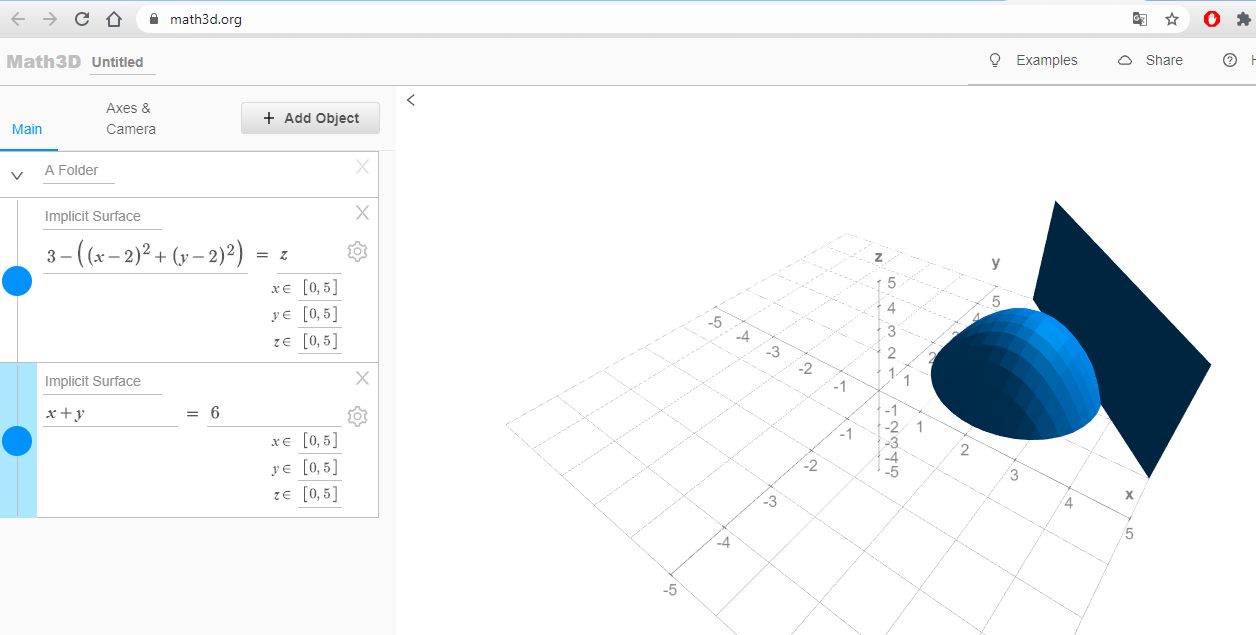
\includegraphics[width=1\textwidth]{1.q_ktc}
\captionof{figure}{A cone-like utility function and a loose budget}
\label{fig:ktc}}

\vspace{2mm}

Try to make some graphs yourself on \href{https://www.math3d.org/}{https://www.math3d.org/}. Always remember your utility is the 
extra dimension (z-axis in Figure \ref{fig:ktc}).



%%%%%%%%%%%%%%%%%%%%%%%%%%%%%%%%%%%%%%%%%%%%%%%%%%%%%%%%%%%%%%%%%%%%%%%%%%%%%%%%%%%%%%%%%%%%%%
\section{Seminar 2}

%***************************************************
\subsection{question 1.}

%%%%%%%%%%%%%%%%%%%%%%%%%%%%%%%%%%%%%%%%%%%%%%%%%%%%%%%%%%%%%%%%%%%%%%%%%%%%%%%%%%%%%%%%%%%%%%
\section{Seminar 7}
\subsection{question 3}

\end{document}
